\documentclass[main.tex]{subfiles}
\begin{document}

\section{Results}
\subsection{Energy Cal}
\begin{figure}[ht]
    \centering
        \includegraphics[width=\textwidth]{DigitalResults/Ecall.png}
        \caption{The digitized energy spectrum.}
    \label{fig:D_QDC}
\end{figure}


\subsection{Time of flight spectrum}
\begin{figure}[ht!]
    \centering
        \includegraphics[width=\textwidth]{DigitalResults/tof.pdf}
        \caption{The time of flight spectrum.}
    \label{fig:D_PSD_TOF} 
\end{figure}

\subsection{Pulse shape discrimination}
\subsubsection{Charge comparisson method}
four parameters to tune: longgate and shortgate window and longgate and shortgate offset. Justify choice!
\begin{figure}[ht!]
    \centering
        \includegraphics[width=\textwidth]{DigitalResults/psd.pdf}
        \caption{Hexbin heatmap of Pulse shape distribution. The upper band is neutrons and the lower one is gammas.}
        \label{fig:hex_a}
\end{figure}
\subsubsection{Convolutional neural network based discrimination}
Show the decision space
\begin{figure}[ht!]
    \centering
        \includegraphics[width=\textwidth]{DigitalResults/tailTotal_vs_cnnPred.png}
        \caption{CNN prediction vs pulse shape. Old dataset!}
    \label{fig:tof_ps_d} 
\end{figure}

\subsection{Pulse shape v ToF and PSD filtered spectra}

\begin{figure}[h!]
    \centering
        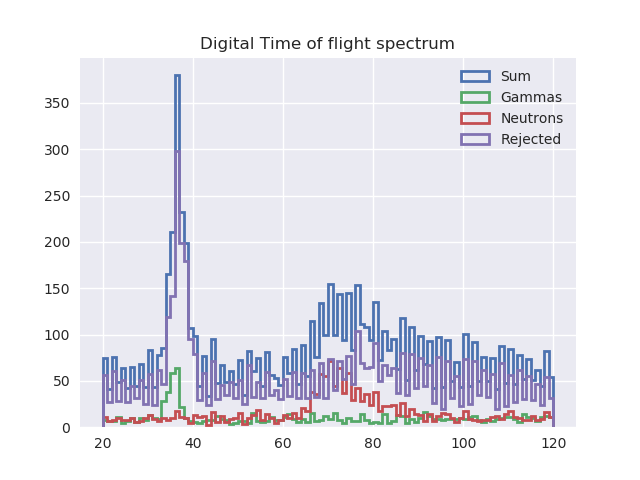
\includegraphics[width=\textwidth]{DigitalResults/tof_psd.pdf}
        \caption{heatmap of ToF vs charge comparisson psd parameter.}
    \label{fig:tof_ps_d} 
\end{figure}

\subsection{Benchmarks}
-$\frac{Livetime}{runtime}$
\newline-explain differences in QDC and ToF spectra
\newline- FoM comparisson
\begin{figure}[h]
    \centering
        \includegraphics[width=\textwidth]{CompareResults/comp.png}
        \caption{The digital energy spectrum.}
    \label{fig:D_QDC}
\end{figure}

\end{document}